\chapter{Results, Discussion and Conclusions}\label{ch:conclusion}

When it comes to testing, two different approaches for building the figures have been addressed in the project. They will be refered throughout the text as \textit{"On the fly"} and \textit{"Regular"} construction.

The \textit{"Regular"} construction consists of the steps described in section \ref{sec:workiing_principle} and it is shown in the first video. 

The second video, which shows the \textit{"On the fly"} construction, differs a bit in some of the steps with the \textit{"Regular"} one.
For starters, this second form of building will only take \textbf{one} picture per figure. This results in a faster construction since taking a new picture and making the whole process to calculate new positions of the blocks every time takes quite a bit of time.
However, this sort of process introduced a new problem to the table. We are choosing the block that is going to be picked based on the maximum area and, in some cases, the same color will have to be picked twice.
For this reason a "color counter" has been added during this method, keeping track of how many times a certain color has been picked and therefore calculating the position of the desired block as the relative maximum area with respect to the counter. I.e.: If one color has to be picked more than once, the block with the second biggest area would be picked the second time, the one with the third biggest area would be picked the third time, and so on. 

On the other hand, even though the \textit{"On the fly"} construction is significantly faster, it is also way less \textbf{robust}. This is due to the fact of taking only one picture per each figure construction. 
We can conclude that a compromise between speed and robustness should be achieved in a real scenario, since new blocks can be added to the workspace while a figure is being constructed or even considering the fact that the first (and only) picture is taken in the process might happen to be of not enough quality (blurred).

\paragraph{} Regarding edge dectection, various methods were tested, being the Canny method the one which proved to give the more satisfactory results. 
However, better results could be achieved by introducing an artificial lighting into our workspace, since this would solve the problem of variations in the threshold parameters, which sometimes lead to not accurate calculations of the block's coordinates.

\paragraph{} A similar test was done to calculate the orientation of the blocks, testing methods that used the boundary boxes of the blocks, or even force brute comparison with a pool of different pictures. Fortunately, the final method chosen that compares the slope of the block's side, proved to be the best compromise between accuracy and computation.

\paragraph{} Using a undistorted image of our workspace significantly improved the precision of our position and orientation calculations. Nevertheless, due to not having a perfect undistortion and the thresholding issue mentioned before, the addition of some offets was in need to correct the small displacements of the gripper. 
The process to choose these offsets was made by positioning the block in the center of the camera field of view and manually moving the robot to the correct location and orientation.

\paragraph{} To sum up, understanding and applying the theoretical concepts presented in the lectures in this project, gave us an insight into the automation and robotic principles and how to combine them with the image processing neccesary to replicate a fairly realistic industrial scenario.

\begin{figure}[H]
	\centering
	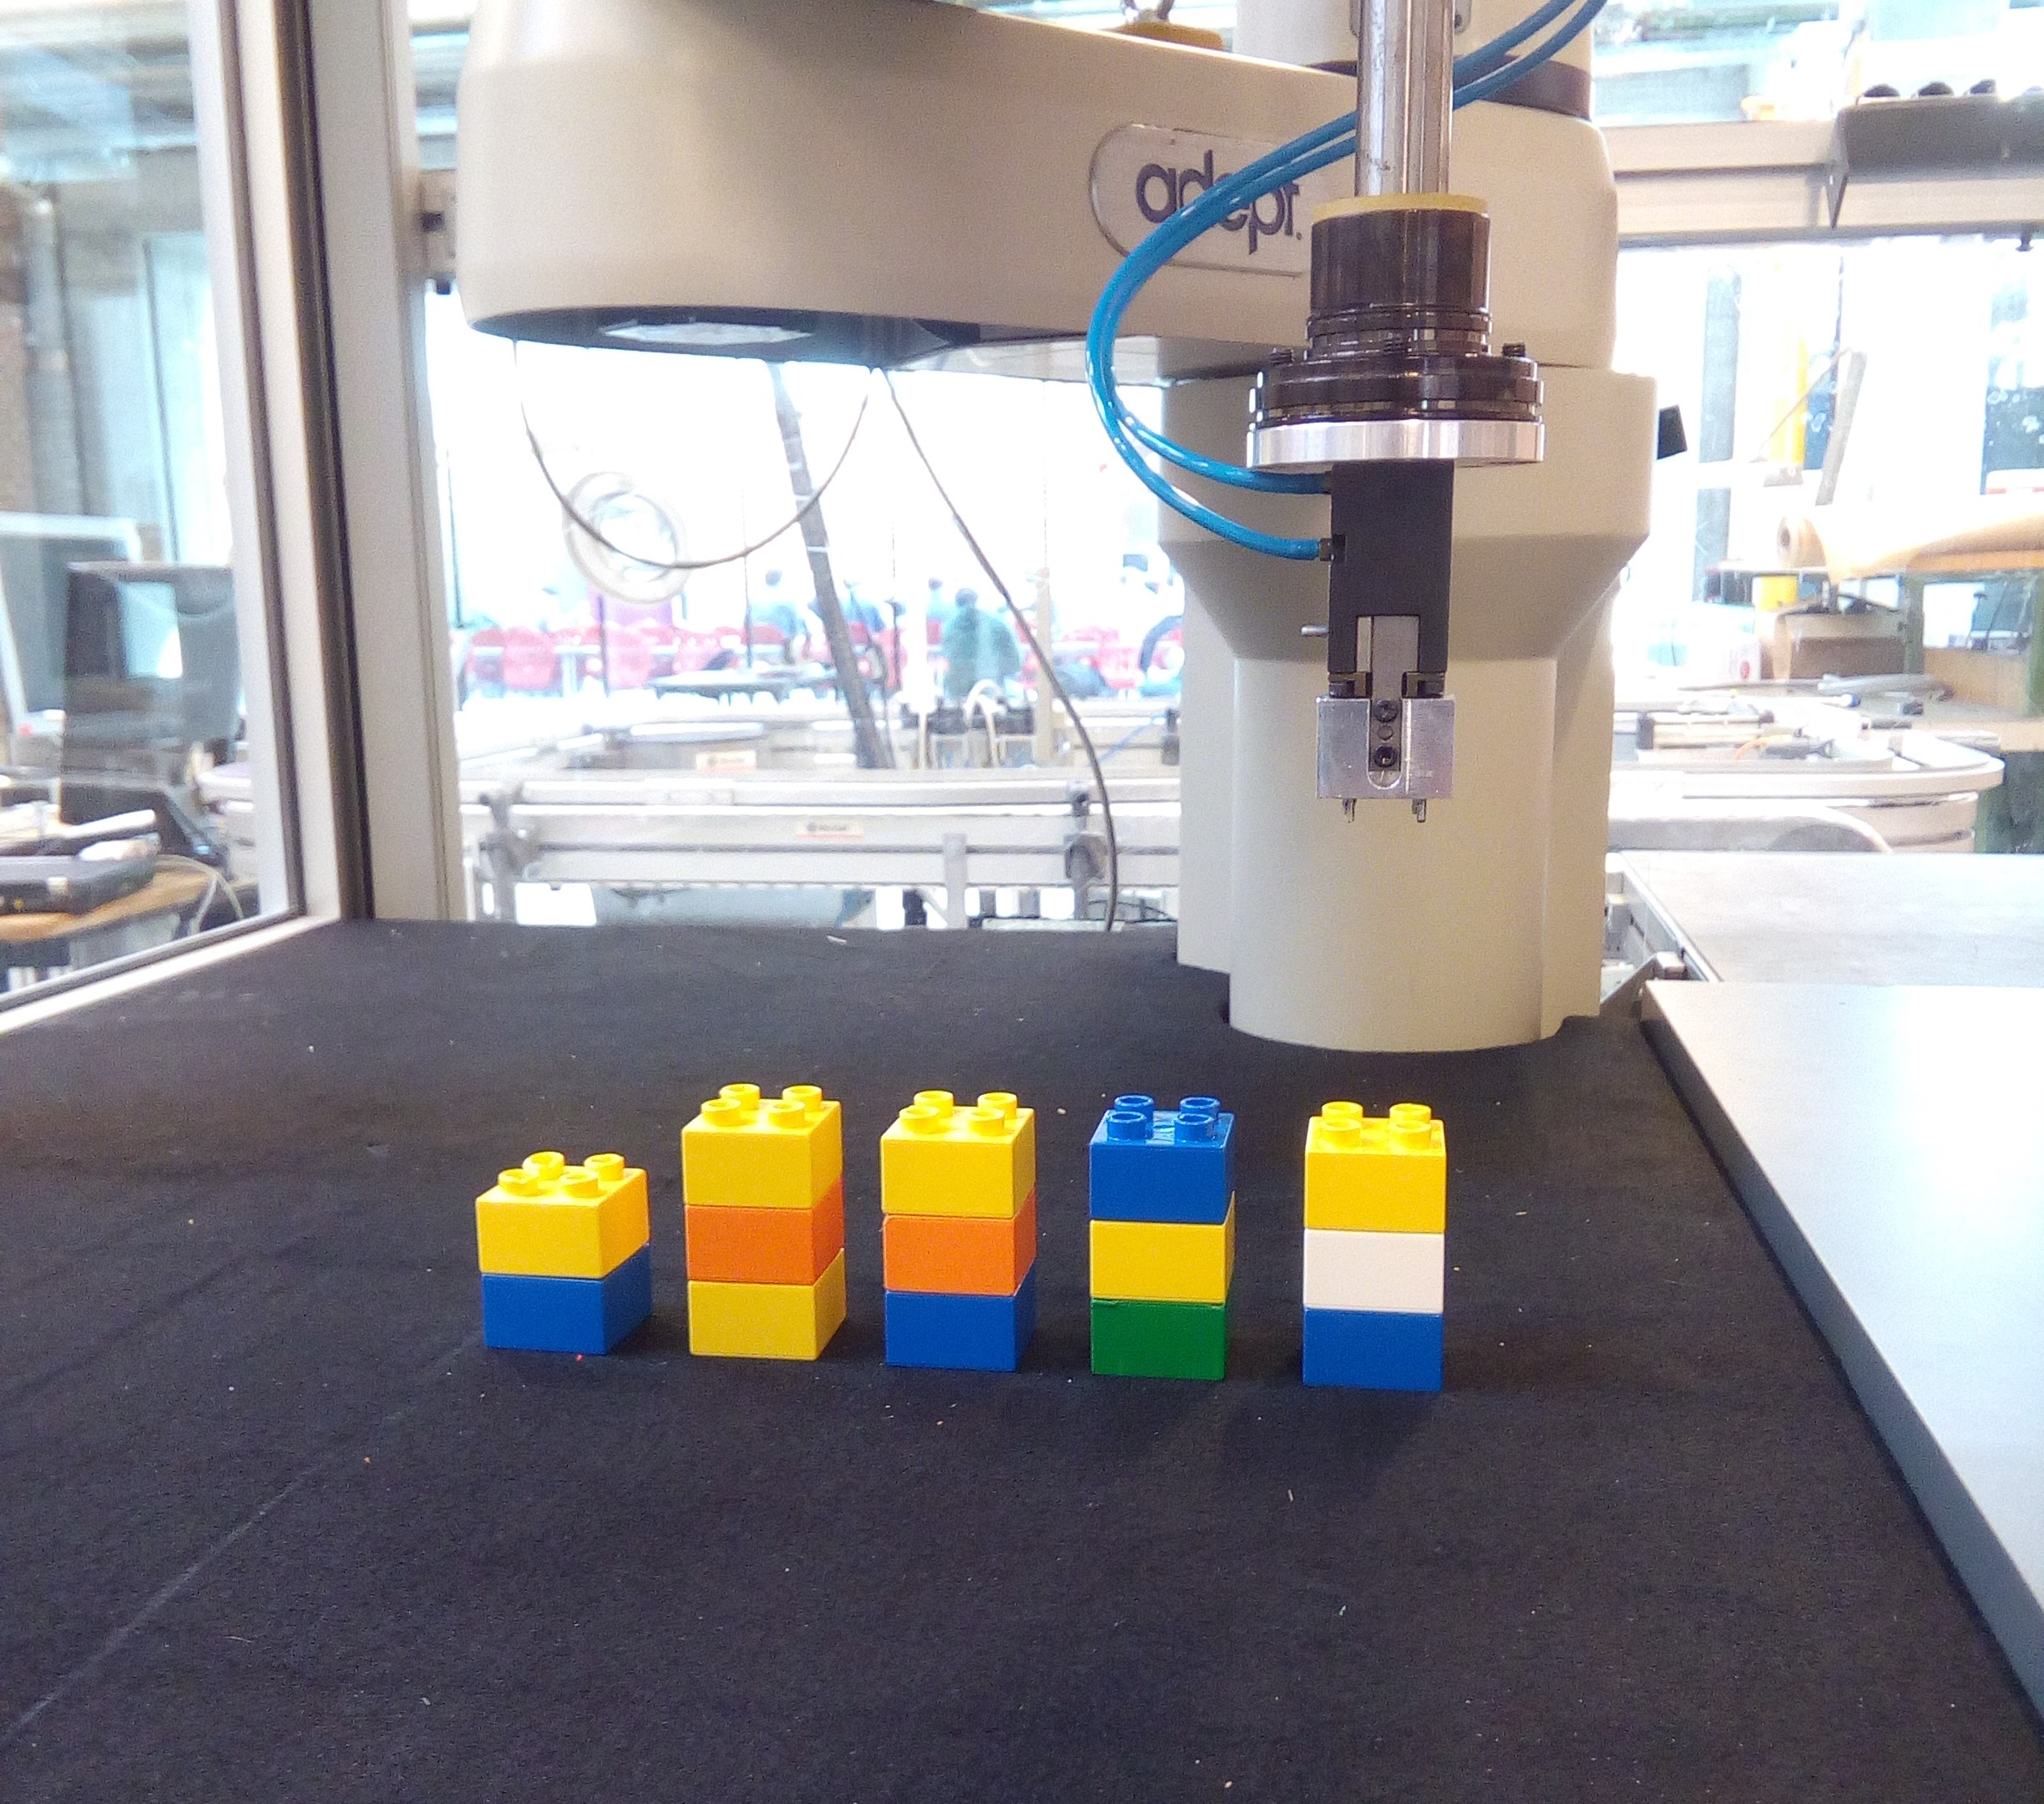
\includegraphics[scale=0.15]{figures/simpsons.jpg}
	\caption{Simpsons Family Picture}
\end{figure}